\section{Results}
\label{sec:results}
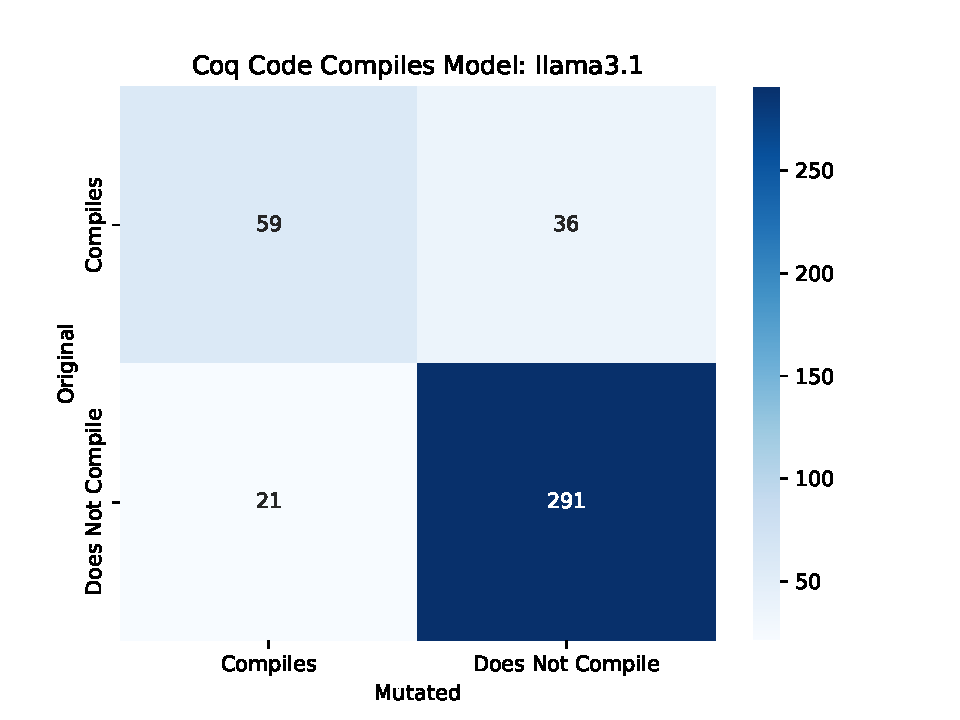
\includegraphics[width=0.5\textwidth]{CM_Compiles_Model_llama3.1}
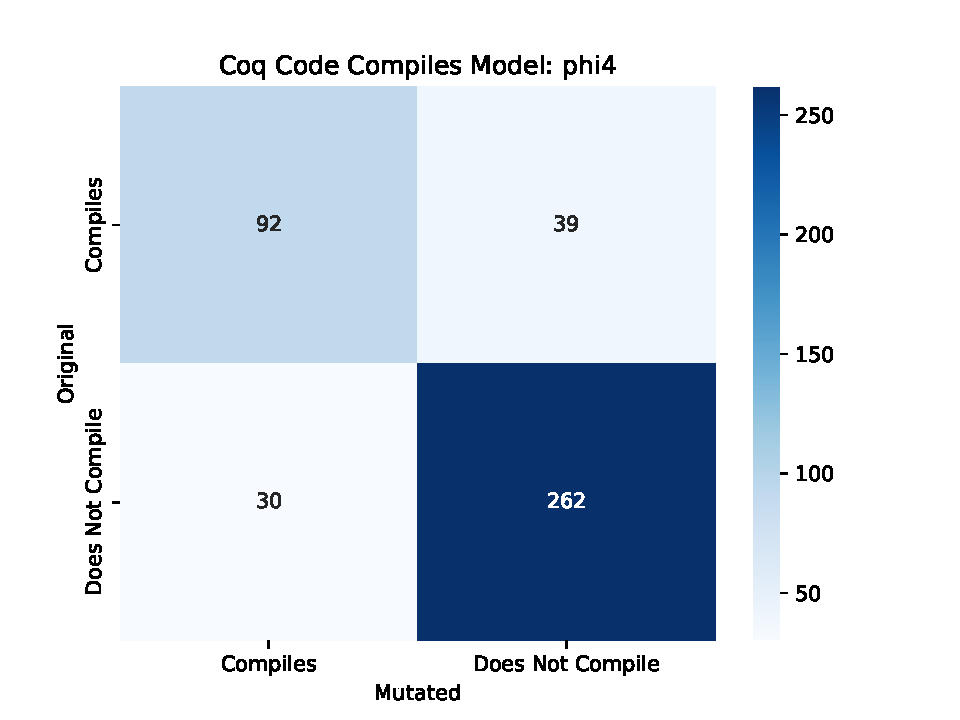
\includegraphics[width=0.5\textwidth]{CM_Compiles_Model_phi4}

Note: failure in the following tables refers to failure to extract a proof from the response (not failure to produce an accepted proof).

\begin{table}[h]
\centering
\begin{tabular}{|l|r|r|r|r|r|}
\hline
\textbf{Model} & \textbf{Entries} & \textbf{Orig. Compile} & \textbf{Mut. Compile} & \textbf{Orig. Fail} & \textbf{Mut. Fail} \\
\hline
llama3.1 & 424 & 22.41 & 19.81 & 3.30 & 0.71 \\
llama3.1 (no failures) & 407& 23.34 & 19.66 & 0.00 & 0.00 \\
phi4 & 424 & 30.90 & 29.01 & 0.24 & 0.00 \\
phi4 (no failures) & 423 & 30.97 & 28.84 & 0.00 & 0.00 \\
\hline
\end{tabular}
\caption{Compilation and failure rates by model (percentages).}
\label{tab:kpi-percentages}
\end{table}

\begin{table}[h]
\centering
\begin{tabular}{|l|r|r|r|r|r|}
\hline
\textbf{Model} & \textbf{Entries} & \textbf{Orig. Compile} & \textbf{Mut. Compile} & \textbf{Orig. Fail} & \textbf{Mut. Fail} \\
\hline
llama3.1 & 424 & 95 & 84 & 14 & 3 \\
llama3.1 (no failures) & 407 & 95 & 80 & 0 & 0 \\
phi4 & 424 & 131 & 123 & 1 & 0 \\
phi4 (no failures) & 423 & 131 & 122 & 0 & 0 \\
\hline
\end{tabular}
\caption{Compilation and failure outcomes by model (counts).}
\label{tab:kpi-counts}
\end{table}

\begin{table}[h]
\centering
\begin{tabular}{|l|c|}
\hline
\textbf{Metric} & \textbf{Value} \\
\hline
Total entries & 848 \\
Total Original Compiles & 226 (26.65\%) \\
Total Original Failed & 15 (1.77\%) \\
Total Mutated Compiles & 207 (24.41\%) \\
Total Mutated Failed & 3 (0.35\%) \\
\hline
\end{tabular}
\caption{Overall basic statistics across all models.}
\label{tab:overall-stats}
\end{table}